\subsection{From Chains to Ledgers}

Blockchain protocols are a type of distributed ledger protocols which includes the three flavors of protocols that we consider.
In blockchain protocols, the ledger is formed using a chain of transaction-containing blocks. Thus, properties of the ledger can be derived from corresponding properties of the chain, which we describe in this section.
We first define temporal blockchain protocols,
a subset of blockchain protocols~\cite{rethinking-consensus}
which keep track of time.

\begin{definition}[(Temporal) Blockchain Protocol]
  A \emph{blockchain} protocol is a distributed protocol
  in which, at the end of every round, each honest party outputs
  a chain. A chain is a finite sequence of blocks. Each block
  contains a finite sequence of transactions.

  A \emph{temporal blockchain} protocol is a blockchain protocol
  where every block contains a recorded round.
\end{definition}

In blockchain protocols, honest parties at every round output a chain
based on their confirmation rule\footnote{
  In longest chain protocols, the output is the longest observed chain without the last $k$ blocks.
  In Streamlet, the output is the longest chain ending in the second of three consecutive notarized
  blocks with consecutive epoch numbers.
} (we also call these \emph{confirmed chains}).
We use $\Chain[][P][r]$ to denote the chain output
by party $P$ at the end of round $r$.

\begin{definition}[Chain Safety]
  A blockchain protocol execution is \emph{safe} if for
  all honest parties $P_1, P_2$ and all rounds $r_1, r_2$,
  it holds that $\Chain[][P_1][r_1] \sim \Chain[][P_2][r_2]$.
  Furthermore, $\Chain[][P_1][r_1] \preccurlyeq \Chain[][P_1][r_2]$ (sticky).
\end{definition}

\noindent
\textbf{From Temporal Blockchains to Temporal Ledgers.}
Any temporal blockchain protocol can be transformed into a
temporal ledger protocol using the following construction:
When \rread is invoked on party $P$ at the end of round $r$, each transaction in
$\Chain[][P][r]$ is reported to $\Ledger[][P][r]$ in the same order as in $\Chain[][P][r]$, and with
the recorded round of the block in which it is included.
We call these protocols \emph{chain-based temporal ledger protocols}.
Note that an execution of the temporal blockchain protocol corresponds to an execution of the chain-based temporal ledger protocol.
Ledger protocols based on safe blockchains are safe.

We now introduce two intermediate properties of temporal blockchains
that will help us prove timeliness of
chain-based temporal ledger protocols.

\begin{definition}[Consistent Recorded Rounds]
  A temporal blockchain protocol execution has \emph{consistent recorded rounds}
  when for all honest parties $P$ and rounds $r$,
  the recorded rounds in $\Chain[][P][r]$ are non-decreasing and not
  in the future.
  Additionally, honestly produced blocks\footnote{
    Abstractly, an honestly produced block is a block that was first
    sent to the network during a broadcast by an honest party. Concretely, in proof-of-work
    and proof-of-stake, these correspond to honestly mined and honestly
    proposed blocks respectively. Genesis is considered honestly produced.
  } record the round during which
  they were produced.
\end{definition}

\begin{definition}[Freshness] \label{def:tip-freshness}
  A temporal blockchain protocol execution is \emph{fresh}($w$) when for
  any round $r$, the recorded round
  $r^*$ of the tip of any honest party's chain output
  satisfies $r - r^* \leq w$.
\end{definition}

The notion of \emph{freshness} tells us that the recorded round
of any confirmed chain tip cannot be more than $w$ rounds old.
Freshness is a \emph{chain} protocol property.
On the other hand, \emph{timeliness} is a \emph{distributed ledger} protocol property,
which tells us that newly appearing transactions
do not have recorded rounds more than $v$ rounds old.
When a ledger protocol is constructed using a chain,
these two notions are related through the following theorem.

\begin{theorem}[Freshness to Timeliness] \label{thm:freshness-to-timeliness}
  An execution of a temporal ledger protocol based on
  temporal blockchain protocol
  whose execution is safe, fresh($w$) and has consistent recorded rounds is timely with timeliness $v = w$.
\end{theorem}
\begin{proof}
  Requirements (1) and (2) of timeliness are directly satisfied from
  the consistent recorded rounds.
  We now prove (3).

  Consider any honest party $P$, and any rounds $r_1 \leq r_2$.
  Suppose, towards a contradiction, that $\Ledger[][P][r_2][|\Ledger[][P][r_1]|{:}]$
  contains a transaction $\tx$ with recorded round $r \leq r_1 - v$.
  Due to chain safety, it holds that $\Chain[][P][r_1] \prec \Chain[][P][r_2]$.
  Transaction $\tx$ is in some block $B \in \Chain[][P][r_2][|\Chain[][P][r_1]|{:}]$
  (see Figure~\ref{fig:freshness-to-timeliness}).
  Let $B^*$ be the tip of $\Chain[][P][r_1]$ with recorded round $r^*$.
  Because of freshness, it holds that $r_1 - r^* \leq w$.
  Therefore, from $r \leq r_1 - v$ it follows that $r - r^* \leq w - v = 0$.

  \begin{figure}
    \centering
    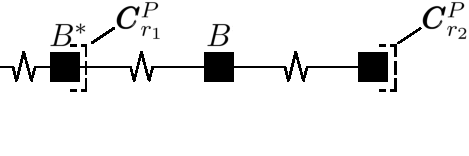
\includegraphics[width=0.5\columnwidth,keepaspectratio]{figures/freshness-timeliness.pdf}
    \caption{The chain in the proof of Theorem~\ref{thm:freshness-to-timeliness}.}
    \label{fig:freshness-to-timeliness}
  \end{figure}

  This is a contradiction because block $B$ extends a chain that contains $B^*$,
  and hence $r > r^*$.
  \Qed
\end{proof}

The following chain property, \emph{recency}, suffices to show freshness\footnote{
  In addition to freshness, recency also suffices to show liveness.
} and is an intermediate property which will be easier to prove.

\begin{definition}[Recency]
  A blockchain protocol execution is \emph{recent}($w$)
  when for any round $r$ and honest party $P$, $\Chain[][P][r]$
  contains a block that was produced by an honest party
  at most $w$ rounds ago.
\end{definition}

Recency directly yields freshness by the following theorem.

\begin{theorem}[Recency to Freshness]\label{thm.recency-to-freshness}
  Temporal Blockchains with consistent recorded rounds and recency($w$) are fresh($w$).
\end{theorem}
\begin{proof}
  Let $P$ be any honest party, $r$ be any round, and
  $r^*$ be the recorded round of the tip $\Chain[][P][r][-1]$.
  From recency, there is a block $B' \in \Chain[][P][r]$
  honestly produced at round $r' \geq r - w$.
  Because of consistent recorded rounds, its recorded round is also $r'$.
  It follows that $r^* \geq r' \geq r - w$.
  \Qed
\end{proof}

In the next subsections, we express Streamlet, Bitcoin and Ouroboros
as chain-based temporal ledger protocols, and we prove that they are recent,
thereby showing they are timely.
